% options:
% thesis=B bachelor's thesis
% thesis=M master's thesis
% czech thesis in Czech language
% slovak thesis in Slovak language
% english thesis in English language
% hidelinks remove colour boxes around hyperlinks

\documentclass[thesis=M,czech]{FITthesis}[2012/06/26]

\usepackage[utf8]{inputenc} % LaTeX source encoded as UTF-8

\usepackage{float}

\usepackage{graphicx} %graphics files inclusion
% \usepackage{amsmath} %advanced maths
% \usepackage{amssymb} %additional math symbols

\usepackage{dirtree} %directory tree visualisation

% % list of acronyms
% \usepackage[acronym,nonumberlist,toc,numberedsection=autolabel]{glossaries}
% \iflanguage{czech}{\renewcommand*{\acronymname}{Seznam pou{\v z}it{\' y}ch zkratek}}{}
% \makeglossaries

\newcommand{\tg}{\mathop{\mathrm{tg}}} %cesky tangens
\newcommand{\cotg}{\mathop{\mathrm{cotg}}} %cesky cotangens

% % % % % % % % % % % % % % % % % % % % % % % % % % % % % % 
% ODTUD DAL VSE ZMENTE
% % % % % % % % % % % % % % % % % % % % % % % % % % % % % % 

\department{Katedra softwarového inženýrství}
\title{Vývoj FIORI aplikace nad SAP PM modulem pro realizaci servisních zakázek a preventivní údržby}
\authorGN{Marcel} %(křestní) jméno (jména) autora
\authorFN{Morávek} %příjmení autora
\authorWithDegrees{Bc. Marcel Morávek} %jméno autora včetně současných akademických titulů
\author{Marcel Morávek} %jméno autora bez akademických titulů
\supervisor{Ing. Martin Šindlář}
\acknowledgements{Poděkování}
\abstractCS{Abstrakt CZ}
\abstractEN{Abstrakt EN}
\placeForDeclarationOfAuthenticity{V~Praze}
\declarationOfAuthenticityOption{4} %volba Prohlášení (číslo 1-6)
\keywordsCS{SAP, Fiori}
\keywordsEN{SAP, Fiori}
% \website{http://site.example/thesis} %volitelná URL práce, objeví se v tiráži - úplně odstraňte, nemáte-li URL práce

\begin{document}

% \newacronym{CVUT}{{\v C}VUT}{{\v C}esk{\' e} vysok{\' e} u{\v c}en{\' i} technick{\' e} v Praze}
% \newacronym{FIT}{FIT}{Fakulta informa{\v c}n{\' i}ch technologi{\' i}}

\begin{introduction}
	Tato práce se zaobírá ...
\end{introduction}

\chapter{Cíl práce}
Cílem této práce je vytvoření webové SAP Fiori aplikace nad SAPovským modulem údržby ve frameworku SAPUI5. Pomocí této aplikace bude umožněno realizovat servisní zakázky i preventivní údržbu strojů a to včetně jejich vybavení.

\section{Rešeršní část}
Jedním z cílů rešeršní části je porovnání prostředí podporujících vývoj ve frameworku SAPUI5. 

\section{Vývojová část}
Cílem praktické části je navržení uživatelského rozhraní aplikace s ohledem na způsob zacházení s modulem údržby. Nadále pak implementace samotné aplikace dle provedeného návrhu. 

\section{Co není cílem práce}

\chapter{SAP PM}
\section{Společnost SAP}
Společnost SAP je v současné době jedním z největších poskytovatelů podnikových aplikací a jednou z největších softwarových společností na celém světe. 
Pod zkratkou SAP se schovávají počáteční písmena německých slov „Systeme, Anwendungen, Produkte in der Datenverarbeitung“. Anglicky si lze zkratku přeložit pomocí anglických slov „Systems - Applications - Products in data processing“.

\section{SAP R3}
Příchodem verze SAP R/3 se změnila architektura SAPu na architekturu klient-server, kte-rá je tvořena třemi vrstvami:
\begin{itemize}
	\item
	\textbf{Prezenční vrstva}
	\item
	\textbf{Aplikační vrstva}
	\item
	\textbf{Databázová vrstva}
\end{itemize} 	

\subsection{Moduly SAP R3}
Systém SAP R/3 je vnitřně rozdělen do několika různých modulů. Každý z nich pak řeší konkrétní problematiku firmy.

\begin{itemize}
	\item
	\textbf{Financial Accounting (FI)} - Finanční účetnictví 
	\item
	\textbf{Controlling (CO)} - Kontroling
	\item
	\textbf{Asset Management (AM)} - Evidence majetku
	\item
	\textbf{Project system (PS)} - Plánování dlouhodobých projektů
	\item
	\textbf{Workflow (WF)} - Řízení oběhu dokumentů
	\item
	\textbf{Industry Solutions (IS)} - Specifická řešení různých odvětví
	\item
	\textbf{Human Resources (HR)} - Řízení lidských zdrojů  
	\item
	\textbf{Plant Maintenance (PM)} - Údržba
	\item
	\textbf{Materials Management (MM)} - Skladové hospodářství a logistika
	\item
	\textbf{Quality Management (QM)} - Management kvality
	\item
	\textbf{Production Planning (PP)} - Plánování výroby 
	\item
	\textbf{Sales and Distribution (SD)} - Podpora prodeje   
\end{itemize} 	

\begin{figure}[H]
	\centering
	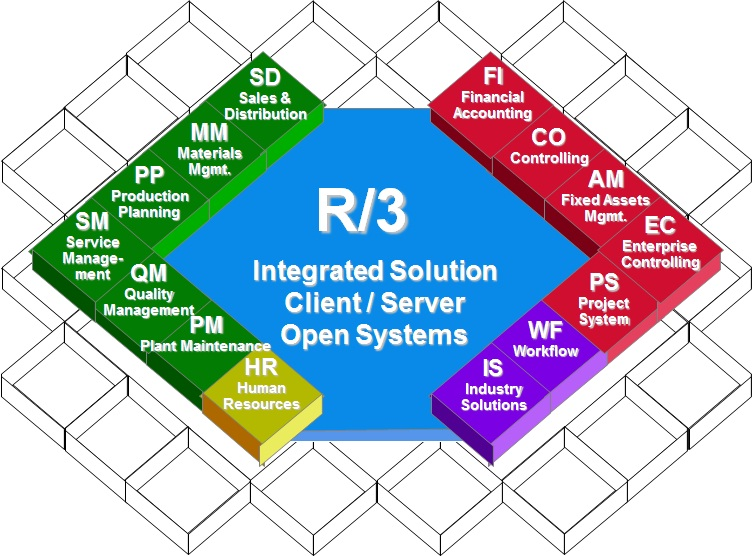
\includegraphics[width=1\textwidth]{images/sap_r3.jpg}
	\caption{Moduly SAP R3}
	\label{img:sapr3}
	\small
	fghfghgddh
\end{figure}

\subsection{SAP Plant Maintenance (PM)}

\chapter{Analýza a návrh aplikace}
Tato kapitola se věnuje analýze mnou navrženého řešení. Obsahuje jednotlivé podkapitoly zaměřující se na zpracování požadavků kladených na výslednou aplikaci, funkčnost RFID čtečky i návrh kompletního třídního modelu.	

\section{Model požadavků}
V této kapitole jsou uvedeny veškeré požadavky kladené na  výslednou aplikaci, které byly probírány se zadavatelem. Většina z nich byla stanovena ihned po určení rámcového zadání, některé však byly přidány nebo lehce upraveny v rámci konzultací , jak se upravovalo zadání práce. Následující výčet požadavků je rozdělen do dvou kategorií a to do funkčních a nefunkčních požadavků.  

\subsection{Funkční požadavky}

\subsubsection{F1: Založení poruchy}
\subsubsection{F2: Založení požadavku na údržbu}
\subsubsection{F3: Zobrazení seznamu aktivních poruch}
\subsubsection{F4: Zobrazení seznamu historie poruch}
\subsubsection{F5: Zobrazení seznamu požadavků na údržbu}
\subsubsection{F6: Zobrazení seznamu prevencí}
\subsubsection{F7: Zobrazení dokumentace ke stroji (vybavení)}
\subsubsection{F8: Administrace uživatele}

\subsection{Nefunkční požadavky}

\subsubsection{N1: Grafické uživatelské rozhraní}
\subsubsection{N2: Provoz na provozních počítačích}
\subsubsection{N3: Provoz na mobilních zařízeních}
\subsubsection{N4: Dostupnost přes web}

\section{Model případů užití (Use Case model)}
Detailní specifikace funkčních požadavků, Typicky se jednotlivé požadavky rozpadají na několik případů užití. Základ pro tvorbu uživatelské příručky
– Podklady k tvorbě akceptačních testů
– Zpřesnění odhadů pracnosti
– Zadání pro programátora


\subsection{Seznam účastníků}

\begin{itemize}
	\item
	\textbf{Operátor výroby} - 
	\item
	\textbf{Údržbář} - 
	\item
	\textbf{Správce - Administrátor} - 
\end{itemize} 	

\subsection{Diagram případů užití}

\subsubsection{UC1: Vložit novou knihu}



\section{Návrh uživatelského rozhraní}

\subsection{Balsamiq}

\subsection{Built}

\chapter{Implementace}

\section{Porovnání vývojových prostředí}

\section{Doporučení pro vývoj}

\begin{conclusion}
	%sem napište závěr Vaší práce
\end{conclusion}

\bibliographystyle{csn690}
\bibliography{mybibliographyfile}

\appendix

\chapter{Seznam použitých zkratek}
% \printglossaries
\begin{description}
	\item[GUI] Graphical user interface
	\item[XML] Extensible markup language
\end{description}


% % % % % % % % % % % % % % % % % % % % % % % % % % % % 
% % Tuto kapitolu z výsledné práce ODSTRAŇTE.
% % % % % % % % % % % % % % % % % % % % % % % % % % % % 
% 
% \chapter{Návod k~použití této šablony}
% 
% Tento dokument slouží jako základ pro napsání závěrečné práce na Fakultě informačních technologií ČVUT v~Praze.
% 
% \section{Výběr základu}
% 
% Vyberte si šablonu podle druhu práce (bakalářská, diplomová), jazyka (čeština, angličtina) a kódování (ASCII, \mbox{UTF-8}, \mbox{ISO-8859-2} neboli latin2 a nebo \mbox{Windows-1250}). 
% 
% V~české variantě naleznete šablony v~souborech pojmenovaných ve formátu práce\_kódování.tex. Typ může být:
% \begin{description}
% 	\item[BP] bakalářská práce,
% 	\item[DP] diplomová (magisterská) práce.
% \end{description}
% Kódování, ve kterém chcete psát, může být:
% \begin{description}
% 	\item[UTF-8] kódování Unicode,
% 	\item[ISO-8859-2] latin2,
% 	\item[Windows-1250] znaková sada 1250 Windows.
% \end{description}
% V~případě nejistoty ohledně kódování doporučujeme následující postup:
% \begin{enumerate}
% 	\item Otevřete šablony pro kódování UTF-8 v~editoru prostého textu, který chcete pro psaní práce použít -- pokud můžete texty s~diakritikou normálně přečíst, použijte tuto šablonu.
% 	\item V~opačném případě postupujte dále podle toho, jaký operační systém používáte:
% 	\begin{itemize}
% 		\item v~případě Windows použijte šablonu pro kódování \mbox{Windows-1250},
% 		\item jinak zkuste použít šablonu pro kódování \mbox{ISO-8859-2}.
% 	\end{itemize}
% \end{enumerate}
% 
% 
% V~anglické variantě jsou šablony pojmenované podle typu práce, možnosti jsou:
% \begin{description}
% 	\item[bachelors] bakalářská práce,
% 	\item[masters] diplomová (magisterská) práce.
% \end{description}
% 
% \section{Použití šablony}
% 
% Šablona je určena pro zpracování systémem \LaTeXe{}. Text je možné psát v~textovém editoru jako prostý text, lze však také využít specializovaný editor pro \LaTeX{}, např. Kile.
% 
% Pro získání tisknutelného výstupu z~takto vytvořeného souboru použijte příkaz \verb|pdflatex|, kterému předáte cestu k~souboru jako parametr. Vhodný editor pro \LaTeX{} toto udělá za Vás. \verb|pdfcslatex| ani \verb|cslatex| \emph{nebudou} s~těmito šablonami fungovat.
% 
% Více informací o~použití systému \LaTeX{} najdete např. v~\cite{wikilatex}.
% 
% \subsection{Typografie}
% 
% Při psaní dodržujte typografické konvence zvoleného jazyka. České \uv{uvozovky} zapisujte použitím příkazu \verb|\uv|, kterému v~parametru předáte text, jenž má být v~uvozovkách. Anglické otevírací uvozovky se v~\LaTeX{}u zadávají jako dva zpětné apostrofy, uzavírací uvozovky jako dva apostrofy. Často chybně uváděný symbol "{} (palce) nemá s~uvozovkami nic společného.
% 
% Dále je třeba zabránit zalomení řádky mezi některými slovy, v~češtině např. za jednopísmennými předložkami a spojkami (vyjma \uv{a}). To docílíte vložením pružné nezalomitelné mezery -- znakem \texttt{\textasciitilde}. V~tomto případě to není třeba dělat ručně, lze použít program \verb|vlna|.
% 
% Více o~typografii viz \cite{kobltypo}.
% 
% \subsection{Obrázky}
% 
% Pro umožnění vkládání obrázků je vhodné použít balíček \verb|graphicx|, samotné vložení se provede příkazem \verb|\includegraphics|. Takto je možné vkládat obrázky ve formátu PDF, PNG a JPEG jestliže používáte pdf\LaTeX{} nebo ve formátu EPS jestliže používáte \LaTeX{}. Doporučujeme preferovat vektorové obrázky před rastrovými (vyjma fotografií).
% 
% \subsubsection{Získání vhodného formátu}
% 
% Pro získání vektorových formátů PDF nebo EPS z~jiných lze použít některý z~vektorových grafických editorů. Pro převod rastrového obrázku na vektorový lze použít rasterizaci, kterou mnohé editory zvládají (např. Inkscape). Pro konverze lze použít též nástroje pro dávkové zpracování běžně dodávané s~\LaTeX{}em, např. \verb|epstopdf|.
% 
% \subsubsection{Plovoucí prostředí}
% 
% Příkazem \verb|\includegraphics| lze obrázky vkládat přímo, doporučujeme však použít plovoucí prostředí, konkrétně \verb|figure|. Například obrázek \ref{fig:float} byl vložen tímto způsobem. Vůbec přitom nevadí, když je obrázek umístěn jinde, než bylo původně zamýšleno -- je tomu tak hlavně kvůli dodržení typografických konvencí. Namísto vynucování konkrétní pozice obrázku doporučujeme používat odkazování z~textu (dvojice příkazů \verb|\label| a \verb|\ref|).
% 
% \begin{figure}\centering
% 	
\includegraphics[width=0.5\textwidth, angle=30]{cvut-logo-bw}
% 	\caption[Příklad obrázku]{Ukázkový obrázek v~plovoucím prostředí}\label{fig:float}
% \end{figure}
% 
% \subsubsection{Verze obrázků}
% 
% % Gnuplot BW i barevně
% Může se hodit mít více verzí stejného obrázku, např. pro barevný či černobílý tisk a nebo pro prezentaci. S~pomocí některých nástrojů na generování grafiky je to snadné.
% 
% Máte-li například graf vytvořený v programu Gnuplot, můžete jeho černobílou variantu (viz obr. \ref{fig:gnuplot-bw}) vytvořit parametrem \verb|monochrome dashed| příkazu \verb|set term|. Barevnou variantu (viz obr. \ref{fig:gnuplot-col}) vhodnou na prezentace lze vytvořit parametrem \verb|colour solid|.
% 
% \begin{figure}\centering
% 	\includegraphics{gnuplot-bw}
% 	\caption{Černobílá varianta obrázku generovaného programem Gnuplot}\label{fig:gnuplot-bw}
% \end{figure}
% 
% \begin{figure}\centering
% 	\includegraphics{gnuplot-col}
% 	\caption{Barevná varianta obrázku generovaného programem Gnuplot}\label{fig:gnuplot-col}
% \end{figure}
% 
% 
% \subsection{Tabulky}
% 
% Tabulky lze zadávat různě, např. v~prostředí \verb|tabular|, avšak pro jejich vkládání platí to samé, co pro obrázky -- použijte plovoucí prostředí, v~tomto případě \verb|table|. Například tabulka \ref{tab:matematika} byla vložena tímto způsobem.
% 
% \begin{table}\centering
% 	\caption[Příklad tabulky]{Zadávání matematiky}\label{tab:matematika}
% 	\begin{tabular}{|l|l|c|c|}\hline
% 		Typ		& Prostředí		& \LaTeX{}ovská zkratka	& \TeX{}ovská zkratka	\tabularnewline \hline \hline
% 		Text		& \verb|math|		& \verb|\(...\)|	& \verb|$...$|		\tabularnewline \hline
% 		Displayed	& \verb|displaymath|	& \verb|\[...\]|	& \verb|$$...$$|	\tabularnewline \hline
% 	\end{tabular}
% \end{table}
% 
% % % % % % % % % % % % % % % % % % % % % % % % % % % % 

\chapter{Obsah přiloženého CD}

%upravte podle skutecnosti

\begin{figure}
	\dirtree{%
		.1 readme.txt\DTcomment{stručný popis obsahu CD}.
		.1 exe\DTcomment{adresář se spustitelnou formou implementace}.
		.1 src.
		.2 impl\DTcomment{zdrojové kódy implementace}.
		.2 thesis\DTcomment{zdrojová forma práce ve formátu \LaTeX{}}.
		.1 text\DTcomment{text práce}.
		.2 thesis.pdf\DTcomment{text práce ve formátu PDF}.
		.2 thesis.ps\DTcomment{text práce ve formátu PS}.
	}
\end{figure}

\end{document}
